\chapter{角动量定理 天体运动}

\section*{A 组}
\vspace{0.3cm}
\textbf{4-1} 如图所示, 质量 $m$ 的小球某时刻具有水平朝右的速度 $v$, 小球相对图示长方形中 $A$, $B$, $C$ 三个顶点的距离分别是 $d_{1}$ , $d_{2}$ , $d_{3}$ , 且有 $d_{2}^{2}=d_{1}^{2}+d_{3}^{2}$ . 试求:

(1) 小球所受重力相对 $A$, $B$, $C$ 的力矩；

(2) 小球相对 $A$, $B$, $C$ 的角动量.

\begin{center}
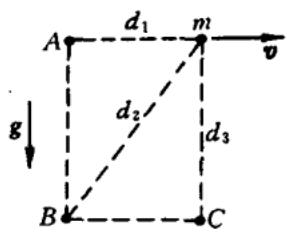
\includegraphics[width=0.2\textwidth]{figures/图4_1.jpg}
\end{center}

\vfill

\textbf{4-2} 质量 $m_{0}$ 的质点固定不动，在它的万有引力作用下，质量 $m$ 的质点作半径为 $R$ 的圆轨道运动。取圆周上 $P$ 点为参考点，如图所示，试求：

(1) 质点 $m$ 在图中点 1 处所受引力的力矩 $M_{1}$ 和质点 $m$ 的角动量 $L_{1}$ ;

(2) 质点 $m$ 在图中点 2 处所受引力的力矩$M_{2}$ 和质点 $m$ 的角动量 $L_{2}$ .


\begin{center}
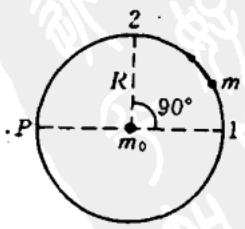
\includegraphics[width=0.2\textwidth]{figures/图4_2.jpg}
\end{center}

\vfill

\newpage

\textbf{4-3} 运动中的某质点, 在惯性系 $S_{1}$ 中相对于任一参考点的角动量都守恒. 试问该质点在惯性系 $S_{2}$ 中, 是否相对于任一参考点的角动量也都守恒? 为什么?


\vfill

\textbf{4-4} 氢原子中的核近似处理为不动, 波尔假设电子绕核作圆轨道运动时, 相对于核的角动量大小必定是 $\hbar = h / 2\pi$ ( $h$ 为普朗克常量) 的整数倍. 将电子质量记作 $m$ , 试导出电子可取的圆轨道半径 $r$ .


\vfill

\newpage

\textbf{4-5} 半径 $R$ 的圆环固定在水平桌面上, 不可伸长的柔软轻细绳全部缠绕在环外侧, 绳末端系一质量 $m$ 的小球, 开始时小球紧贴圆环. $t = 0$ 时刻使小球获得背离环心的水平速度 $\pmb{v}$ , 于是细绳从环外侧打开. 设打开过程中细绳始终处于伸直状态, 且与环间无相对滑动, 小球与桌面间无摩擦.

(1) 计算 t>0 时刻小球相对环心的角动量 $L$;

(2) 利用小球的运动, 验证质点角动量定理.


\vfill

\textbf{4-6} 如图所示, 在半顶角为 $\phi$ 的倒立固定圆锥面光滑内壁上, 一小球在距锥顶 $h_{0}$ 高度处作水平圆周运动.

(1) 试求圆运动速率 $v_{0}$ ;

(2) 若在某时刻, 小球的速度不改变方向地从 $v_{0}$ 增为 $\sqrt{1 + \alpha} v_{0}$ , 其中 $\alpha > 0$ , 小球随即离开原轨道但不会离开锥面内壁, 试问小球是否会在距离锥顶某个 $h$ 高度处作水平圆周运动?

(3) 接(2)问, 小球若不再作圆周运动, 试求运动过程中相对锥顶能达到的最大高度 $h_{max}$ 和最低高度 $h_{min}$ .


\begin{center}
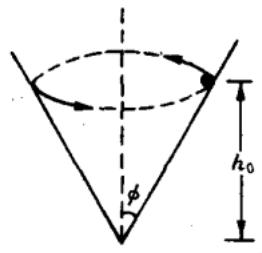
\includegraphics[width=0.2\textwidth]{figures/图4_4.jpg}
\end{center}

\vfill

\newpage

\textbf{4-7} 半径 $R$，用轻辐条支撑的匀质圆环，可绕中央水平轴无摩擦地转动，开始时旋转角速度为 $\omega_{0}$ ，如图所示。而后，将转轴向下移动，直到圆环重力全部都由水平地面支持力抵消为止，并将转轴固定。已知环与地面间的摩擦因数为 $\mu$ ，试问经多长时间停止转动？

\begin{center}
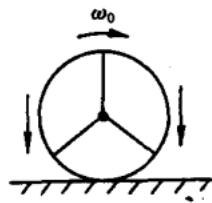
\includegraphics[width=0.2\textwidth]{figures/图4_5.jpg}
\end{center}

\vfill

\textbf{4-8} 设想全世界所有的人都在赤道上自西向东，以接近百米世界记录的速度跑步,试估算地球日长将增长还是缩短多少秒?已知质量 $m$、半径 $R$ 的匀质球绕其直径以角速度 $\omega$ 旋转时,相对球心的角动量为 $\frac{2}{5}mR^{2}\omega$ .


\vfill

\newpage

\textbf{4-9} 如图所示, 光滑的水平大台面绕着过中央 $O$ 点的竖直固定轴逆时针方向匀速旋转, 角速度为 $\omega$ . 台面上的一个固定点 $P$ 与 $O$ 相距 $b$, 在 $P$ 点连接长 $l$ 的轻线, 线的另一端系一小球 $Q$, $Q$ 的稳定平衡位置在 $O$ 与 $P$ 连线上. 设轻线始终处于伸直状态, 小球在台面上作圆弧运动, 引入从平衡位置逆时针方向取正的转角 $\theta$ , 试求角加速度 $\beta$ 与角 $\theta$ 之间的关系.

\begin{center}
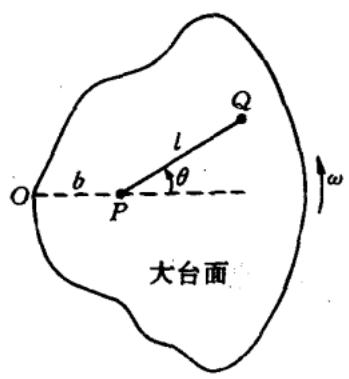
\includegraphics[width=0.2\textwidth]{figures/图4_6.jpg}
\end{center}

\vfill

\textbf{4-10} 质量同为 $m$ 的两个小球系于一轻弹簧两端后，放在光滑水平桌面上，弹簧处于自由长度状态，长为 $a$ ，它的劲度系数为 $k$ 。今使两球同时受水平冲量作用，各获得与连线垂直的等值反向初速度，如图所示. 若在以后运动过程中弹簧可达的最大长度 b=2a，试求两球初速度大小 $v_{0}$ .

\begin{center}
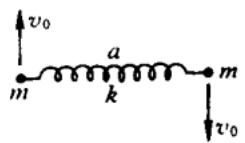
\includegraphics[width=0.25\textwidth]{figures/图4_8.jpg}
\end{center}

\vfill

\newpage

\textbf{4-11} 光滑水平桌面上有一轻质细杆,杆可绕着过中心 $O$ 点的竖直轴无摩擦地转动.有四个质量相同的小球,其中两个分别固定在细杆两端 $A_{1}$ 和 $A_{2}$ 处,另外两个穿在细杆上可沿杆无摩擦自由滑动,它们的初始位置分别在 $OA_{1}$ 和 $OA_{2}$ 的中点.今使系统在极短时间内获得绕 $O$ 轴转动角速度,而后让其自由运动,可动小球将沿杆朝固定小球撞去,试求动球相对细杆初始径向加速度与最后和固定球碰前瞬间径向加速度的比值.


\vfill

\textbf{4-12} (1) 若一个静止地处于平衡状态的物体所受 $N \geqslant 3$ 个外力中, 有 $N - 1$ 个是共点力, 试证这全部 $N$ 个力是共点力.

(2) 半径 $R$ 的光滑圆环固定在某竖直平面内，三边长分别为 $R, \sqrt{3}R, 2R$ 的匀质三角板放在环内，静止地处于平衡状态，如图所示，试求三角板 2R 长边与圆环水平直径间的夹角 $\theta$ .

\begin{center}
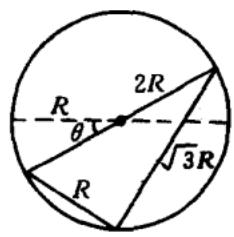
\includegraphics[width=0.2\textwidth]{figures/图4_10.jpg}
\end{center}

\vfill

\newpage

\textbf{4-13} 无动力航天器从远处以初速 $\pmb{v}_0$ 朝质量 $M$ 、半径 $R$ 的行星飞去，行星中心 $O$ 到 $\pmb{v}_0$ 方向线的距离称为瞄准距离，记为 $b$ . $b \leqslant R$ 时，航天器可落到行星表面，即被行星俘获. $b > R$ 时由于万有引力作用，航天器也可能如图所示，落在行星表面，被行星俘获.

(1) 计算航天器可被行星俘获的瞄准距离最大可取值 $b_{0}$ ;

(2) 初速率为 $v_{0}$ 的航天器, 在远处只要瞄准正前方以行星中心$O$ 为心, $b_{0}$ 为半径的几何靶上任何一点飞去,都会被行星俘获,故称 $S=\pi b_{0}^{2}$ 为行星的俘获截面,试求 $S$.

\begin{center}
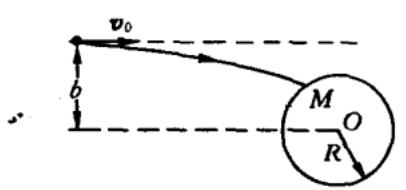
\includegraphics[width=0.3\textwidth]{figures/图4_11.jpg}
\end{center}

\vfill

\textbf{4-14} 从地球表面以第一宇宙速度朝着与竖直方向成 $\alpha$ 角的方向发射一物体, 忽略空气阻力和地球转动的影响, 试问物体能上升多高?

\vfill

\newpage

\textbf{4-15} 小行星 1 和 2 的质量相同, 小行星 1 绕太阳的轨道是一个圆. 小行星 2 绕太阳的轨道是一个非圆的椭圆. 已知圆半径恰好等于椭圆半长轴, 试比较两者轨道能量的大小.


\vfill

\textbf{4-16} 小行星抛物线轨道方程可表述成 $y^{2}=2px$ ，太阳位于焦点 x=p/2, y=0 处。将太阳质量记为 $M$，试求小行星在抛物线顶点处的速度 $v_{0}$ 。

\vfill

\newpage

\textbf{4-17} 某彗星受其他星体引力干扰后进入双曲线轨道，已知双曲线参量 $a$, $b$，彗星和太阳质量分别记为 $m$ 和 $M$，试求彗星近日点速度 $v_{D}$ 和轨道能量 $E$.


\vfill

\textbf{4-18} 1994年7月16日20时15分，哈勃望远镜观察到了休梅克-列维9号彗星的第一块碎片与木星相撞，而后其他碎片相继与木星相撞，直至7月22日8时12分才告结束.

在这之前彗星早已开始绕木星作椭圆运动,据天文测量数据绘制的轨道如图所示,请估算彗星碎片刚进入木星大气层时相对木星的速度大小.

\begin{center}
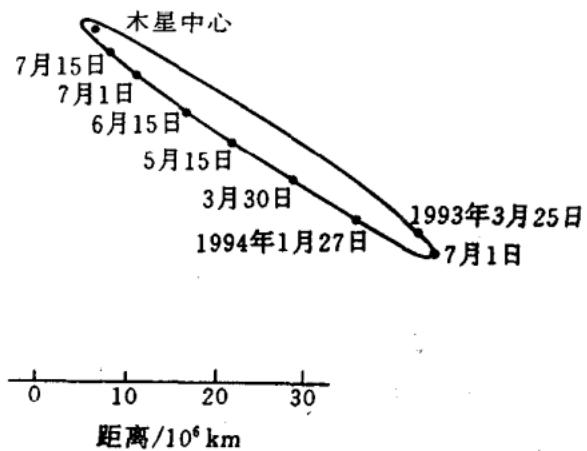
\includegraphics[width=0.3\textwidth]{figures/图4_15.jpg}
\end{center}

\vfill

\newpage

\textbf{4-19} 质量分别为 $m_{1}, m_{2}$ 的两个质点相距 $l$ ，开始时均处于静止状态，其间仅有万有引力相互作用。

(1) 假设 $m_{1}$ 固定不动, $m_{2}$ 将经多长时间后与 $m_{1}$ 相碰?

(2) 假设 $m_{1}$ 也可动, 两者将经多长时间后相碰?

\vfill

\textbf{4-20} 一陨石在地表上方高为 $h = 4.2 \times 10^{3} \mathrm{~km}$ 的圆形轨道上绕地球运动, 它突然与另一质量小得多的小陨石发生正碰, 碰后损失掉 $2\%$ 的动能. 假定碰撞不改变大陨石的运动方向和质量, 试求大陨石在碰撞后最接近地心的距离. 地球半径取为 $R = 6.4 \times 10^{3} \mathrm{~km}$ .


\vfill

\newpage

\textbf{4-21} 行星绕着恒星 $S$ 作圆周运动, 设 $S$ 在很短时间内发生爆炸, 通过强辐射流使其质量减少为原质量 $\gamma$ 倍, 行星随即进入椭圆轨道绕 $S$ 运行, 试求椭圆偏心率 $e$.

\vfill

\textbf{4-22} 宇宙飞船在距火星表面 $H$ 高度处作匀速圆周运动, 火星半径记为 $R$. 设飞船在极短时间内向外侧点火喷气, 使其获得一径向速度, 大小为原速度 $\alpha$ 倍, $\alpha$ 很小, 飞船新轨道不会与火星表面交会.飞船喷气质量可略.

(1) 计算飞船新轨道近火星点高度 $h_{1}$ 和远火星点高度 $h_{2}$ ;

(2) 设飞船原来的运行速度大小为 $v_{0}$ ，计算新轨道运行周期 $T$.

\vfill

\newpage

\section*{B 组}
\vspace{0.3cm}
\textbf{4-23} 以圆锥摆摆球为讨论对象,取悬挂点为参考点,验证质点角动量定理.

\vfill

\textbf{4-24} 质量均为 $m$ 的小球 1,2 用长 $4a$ 的柔软轻细线相连，同以速度 $v$ 沿着与线垂直的方向在光滑水平面上运动，线处于伸直状态。在运动过程中，线上距离小球 1 为 $a$ 的一点与固定在水平面上的竖直光滑细钉相遇，如图所示。设在以后的运动过程中两球不相碰，试求：

(1) 小球 1 与钉的最大距离(给出 4 位有效数字);

(2) 线中的最小张力.

\begin{center}
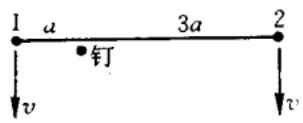
\includegraphics[width=0.3\textwidth]{figures/图_4_20.jpg}
\end{center}

\vfill

\newpage

\textbf{4-25} 光滑水平面上有一小孔, 轻细线穿过小孔, 两者间无摩擦. 细线一端连接质量 $m_{1}$ 的小球, 另一端在水平面下方连接质量 $m_{2}$ 的小球, $m_{1}$ 绕小孔作半径 $r_{0}$ 的圆周运动时, $m_{2}$ 恰好处于静止状态, 如图所示.

(1) 试求 $m_{1}$ 圆运动角速度 $\omega_{0}$ .

(2) 假设 $m_{1}$ 有径向小扰动, $m_{2}$ 有相应的竖直方向小扰动, 此时可将 $m_{1}$ 与孔的距离表述成 $r(t)=r_{0}+\delta(t)$ , 其中 $\delta(t)$ 是随时间变化的小量. 试证 $\delta$ 随 $t$ 的变化是简谐振动, 并导出振动角频率 $\omega_{\delta}$ 与 $\omega_{0}$ 间的比值.

\begin{center}
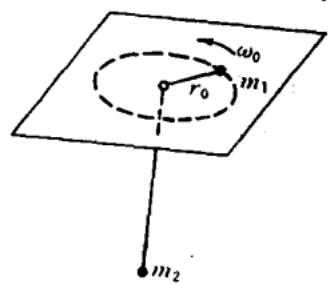
\includegraphics[width=0.3\textwidth]{figures/图4_22.jpg}
\end{center}

\vfill

\textbf{4-26} 约束在某参考系 $xy$ 平面上运动的质点系, 任一时刻动量记作 $\pmb{p}$ . 试证:

(1) 若 p=0，则该时刻质点系相对 xy 平面上所有参考点的角动量相同；

(2) 若 $p \neq 0$ ，则在 xy 平面上必有一条相应的瞬时直线，使得该时刻质点系相对此直线上任何一点的角动量都是零。


\vfill

\newpage

\textbf{4-27} 如图所示, 在光滑的水平面上有一个固定的光滑大圆环, 一个小的发射装置 $P$ 紧贴在圆环的内侧, 开始时处于静止状态, 且头部朝右, 尾部朝左. $P$ 内存有许多微小的光滑珠子, 其总质量与空的发射装置质量相同. 某时刻起, $P$ 从其尾部不断向后发射小珠子, 因珠子微小, 发射可以认为是连续进行的. 设珠子射出时相对 $P$ 的速率为常量, 单位时间发射的珠子质量也是常量; 再设当 $P$ 的头部与前方运动过来的第一个珠子相遇时, $P$ 刚好将其中的珠子全部发射完毕.

(1) 试求 $P$ 在发射珠子的全过程中, $P$ 相对圆环转过的总角度 $\theta$ (精确到 $1^{\circ}$ );

(2) 若 $P$ 的头部遇到前方运动过来的珠子时, 能将珠子吞入其中且不再发射, 试确定 $P$ 相对圆环的最终运动速率 $v_{e}$ .

\begin{center}
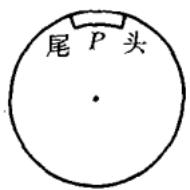
\includegraphics[width=0.2\textwidth]{figures/图4_25.jpg}
\end{center}

\vfill

\textbf{4-28} 质量相同的两个小球 $A_{1}$ 和 $A_{2}$ 固连在一根轻杆两端，轻杆中点 $O$ 固连在一水平轻轴上，轻杆与轻轴夹一锐角. 以 $O$ 为原点建立 Oxyz 坐标系, 其中 $x$ 轴位于轻轴的中央轴线上, 轻轴夹在两个固定的光滑水平轴承内, 可无摩擦地绕 $x$ 轴旋转. 今使 $A_{1}, A_{2}$ 分别在图 4-27 所示两个平行的竖直平面内作匀速圆周运动, 试问由 $A_{1}, A_{2}$ , 轻杆和轻轴构成的系统相对 $O$ 点的角动量是否守恒? 若不守恒, 定性说明相对 $O$ 点提供非零力矩的是哪些力?

\begin{center}
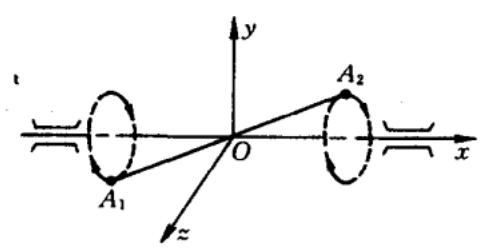
\includegraphics[width=0.35\textwidth]{figures/图4_27.jpg}
\end{center}

\vfill

\newpage

\textbf{4-29} 五根相同的匀质细杆,用质量与线度均可忽略的光滑铰链两两首尾相接连成一个五边形,将其一个顶点悬挂在天花板下,试求平衡时此五边形的五个顶角.(给到0.1°)

又若在最下边的细杆中点再悬挂一重物,能否使五根细杆构成一个等腰三角形?

\vfill

\textbf{4-30} 在行星的轨道运动中引入隆格-楞茨(Runge-Lenz)矢量
\[
\boldsymbol {B} = \boldsymbol {v} \times \boldsymbol {L} - G M m \frac {\boldsymbol {r}}{r},
\]
其中 $M$ 是太阳质量，$m$,$r$,$v$,$L$ 分别是行星的质量、相对于太阳的径矢、速度和角动量.

(1) 试证 $B$ 是个守恒量, 即必有 $\frac{dB}{dt}=0$ ;

(2) 试证 $B^{2} = G^{2}M^{2}m^{2} + \frac{2EL^{2}}{m}$ ;

(3) 试证 $r \cdot B = \frac{L^{2}}{m} - GMmr$ ;

(4) 导出极坐标系中的行星轨道方程.

\vfill

\newpage

\textbf{4-31} 质量为 $M$ 的宇航站和质量为 $m$ 的飞船对接后，一起沿半径为 $nR$ 的圆形轨道绕地球运动，这里的 $n = 1.25, R$ 为地球的半径。而后飞船又从宇航站沿运动方向发射出去，并沿某椭圆轨道飞行，其最远点到地心的距离为 $8nR$ ，宇航站的飞行轨道也变成一椭圆。如果飞船绕地球运行一周后恰好与宇航站相遇，则质量比 $m / M$ 应为何值？


\vfill

\textbf{4-32} 如图所示, 质量 $m=1.20 \times 10^{4}$ kg 的飞船在距月球表面高度 h=100 km 处绕月球作圆运动. 飞船采用两种登月方式:

(1) 在 $A$ 点向前短时间喷气, 使飞船与月球相切地到达月球上的 $B$ 点; (2) 在 $A$ 点向外侧沿月球半径短时间喷气, 使飞船与月球相切地到达月球上的 $C$ 点. 设喷气相对原飞船的速度为 $u = 1.00 \times 10^{4} \, m/s$ . 已知月球半径 $R$ = 1700 km, 月球表面重力加速度 $g = 1.700 \, m/s^{2}$ . 试求两种登月方式各需要的燃料质量.

\begin{center}
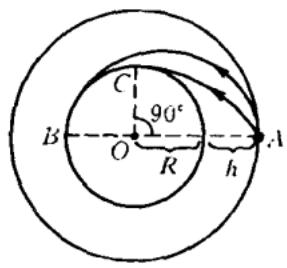
\includegraphics[width=0.2\textwidth]{figures/图4_32.jpg}
\end{center}

\vfill

\newpage

\textbf{4-33} 一质量为 $m$ 的行星绕质量为 $M$ 的恒星运动, 设在以恒星为球心的球形大空间范围内均匀地分布着稀薄的宇宙尘埃, 尘埃的密度 $\rho$ 很小, 可以略去行星与尘埃之间的直接碰撞作用.

(1) 试问, 对于角动量为 $L$ 的圆形行星轨道, 其半径 $r_{0}$ 应满足什么方程(列出方程即可, 不必求解)?

(2) 考虑对上述圆轨道稍有偏离的另一轨道, 试解释它是一条作进动的椭圆轨道, 进动方向与行星运行方向相反, 并求出进动角速度 (用 $r_0$ 表述).

\vfill
